\documentclass{ximera}

\usetikzlibrary{hobby}

\graphicspath{{./graphics/}}

\title{Chain Rule}
\author{Melissa Lynn}
\outcome{Understand and apply the chain rule.}

\begin{document}
\begin{abstract}
\end{abstract}
\maketitle

We'll begin by recalling the chain rule from single variable calculus. If we have differentiable functions $f$ and $g$, then we can compute the derivative of the composition as $(f\circ g)'(x) =f'(g(x))g'(x)$.

\begin{example}
Let $f(x) = \sin(x)$ and $g(x) = x^2$. Then $f'(x) = \cos(x)$, $g'(x)=2x$, and we can differentiate the composition $(f\circ g)(x) = \sin(x^2)$ using the chain rule:
\begin{align*}
(f\circ g)'(x) &= f'(g(x))g'(x)\\
&=\cos(g(x))\cdot 2x\\
&=\cos(x^2)\cdot 2x.
\end{align*}
We can also use the chain rule to differentiate the composition $(g\circ f)(x) = \sin^2(x)$.
\begin{align*}
(g\circ f)'(x) &= g'(f(x))f'(x)\\
&=2(f(x))\cos(x)\\
&=2\sin(x)\cos(x)
\end{align*}
\end{example}
 
\section*{The Chain Rule} 
 
 The multi-variable chain rule is similar, with the derivative matrix taking the place of the single variable derivative, so that the chain rule will involve matrix multiplication. We also need to pay extra attention to whether the composition of functions is even defined.
 
 In particular, suppose we have functions $\vec{g}:\mathbb{R}^m\rightarrow\mathbb{R}^p$ and $\vec{f}:\mathbb{R}^q\rightarrow\mathbb{R}^n$. In order for the composition $\vec{f}\circ \vec{g}$ to be defined, the outputs of $\vec{g}$ need to be sensible inputs for $\vec{f}$. This means that we would need $p=q$, so that $\mathbb{R}^p = \mathbb{R}^q$.
 
 If $\vec{f}$ isn't defined on all of $\mathbb{R}^p$, so that $\vec{f}:X\subset \mathbb{R}^p\rightarrow\mathbb{R}^n$, then the range of $\vec{g}:\mathbb{R}^m\rightarrow\mathbb{R}^p$ would need to be contained in $X$, in order for the composition $\vec{f}\circ\vec{g}$ to be defined. Alternatively, we could restrict the domain of $g$ to ensure that the range of $g$ is contained in the domain of $f$.
 
 \begin{image}
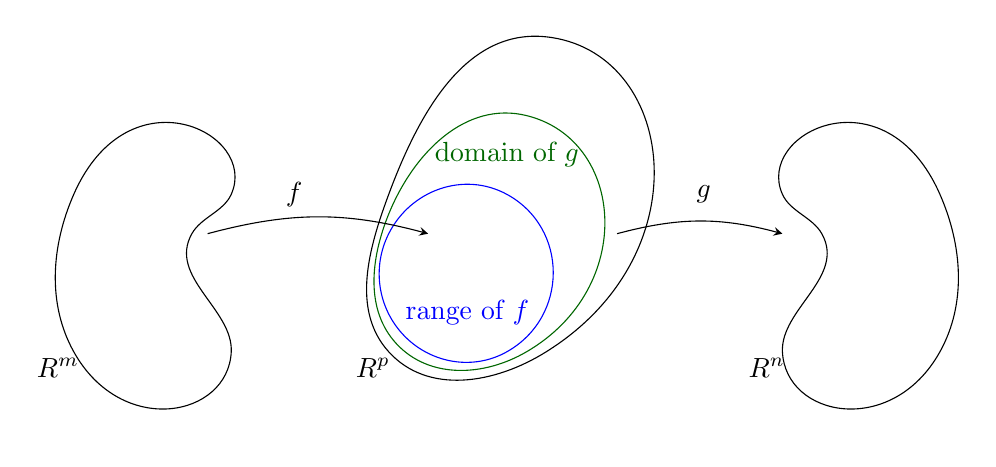
\begin{tikzpicture}
%% first
\path[draw,use Hobby shortcut,closed=true]
(0,0) .. (0,2) .. (2,2) .. (1.5,1.5) .. (2,0);
\node at (-.2,-.2) {$\mathbb{R}^m$};
%% second
\begin{scope}[xshift=4cm]
\node at (-.2,-.2) {$\mathbb{R}^p$};
\path[draw, use Hobby shortcut,closed=true]
(0,0) ..  (0,2) .. (2,4) .. (2,0);
\path[draw, color = black!60!green, use Hobby shortcut,closed=true]
(.1,.1) ..  (0,1.75) .. (1.75,3) .. (1.75,0);
\node[color = black!60!green] at (1.5,2.5) {domain of $g$};
\path[draw, color = blue, use Hobby shortcut,closed=true]
(.2,.2) ..  (0,1.5) .. (1.5,2) .. (1.5,0);
\node[color = blue] at (1,.5) {range of $f$};
\end{scope}
%%third
\begin{scope}[xshift=9cm]
\path[draw,use Hobby shortcut,closed=true]
(2,0) .. (2,2) .. (0,2) .. (.5,1.5) .. (0,0);
\node at (-.2,-.2) {$\mathbb{R}^n$};
\end{scope}
%% arrows
\node at (2.8,2) {$f$};
\path[draw]
(1.7, 1.5) edge[out=15,in=165,-stealth] (4.5,1.5);
\node at (8,2) {$g$};
\path[draw]
(6.9, 1.5) edge[out=15,in=165,-stealth] (9,1.5);
\end{tikzpicture}
\end{image}
 
 \begin{theorem}
 Suppose $\vec{f}:Y\subset\mathbb{R}^p\rightarrow\mathbb{R}^n$ and $\vec{g}:X\subset\mathbb{R}^m\rightarrow\mathbb{R}^p$ are defined on open sets $Y\subset\mathbb{R}^p$ and $X\subset\mathbb{R}^m$, respectively. Suppose that $\vec{g}(X)\subset Y$, so the image of $\vec{g}$ is contained in the domain of $\vec{f}$. Suppose further that $\vec{g}$ is differentiable at some point $\vec{x}_0\in X$, and that $\vec{f}$ is differentiable at $\vec{y}_0=\vec{g}(\vec{x}_0)\in Y$.
 
 Then the composition $\vec{f}\circ\vec{g}$ is differentiable at $\vec{x}_0$, and 
 \begin{align*}
 D(\vec{f}\circ\vec{g})(\vec{x}_0) &= D\vec{f}(\vec{y}_0)D\vec{g}(\vec{x}_0)\\
 &= D\vec{f}(\vec{g}(\vec{x}_0))D\vec{g}(\vec{x}_0).
 \end{align*}
 \end{theorem}
 
 Although the conditions sound complicated, essentially they're just requiring that all of the derivatives mentioned actually exist. Note the similarities to the single variable chain rule.

\section*{A Special Case}

We'll now consider a special case of the chain rule, when we have a composition $f\circ g$ of functions $f:\mathbb{R}^n\rightarrow\mathbb{R}$ and $\vec{g}:\mathbb{R}\rightarrow\mathbb{R}^n$. Note that $f$ is a scalar function, and we can think of $\vec{g}$ as a curve in $\mathbb{R}^n$.

Let's look at what the chain rule tells us in this case. For any $x_0\in\mathbb{R}$, we have
\[ 
D(f\circ\vec{g})(x_0) = Df(\vec{g}(x_0))D\vec{g}(x_0).
\]
Writing $\vec{g}(x) = (g_1(x),...,g_n(x))$ in terms of its components, we have
\[
D\vec{g} = \left(\begin{array}{c}\partial g_1/\partial x\\ \vdots\\\partial g_n/\partial x\end{array}\right).
\]
Since $\vec{g}$ only has one input variable, we can rewrite this as
\[
D\vec{g}(x) = \left(\begin{array}{c}g_1'(x)\\ \vdots\\g_n'(x)\end{array}\right).
\]
Now that we've sorted out $D\vec{g}$, let's consider $Df$. Since $f$ is a scalar-valued function, $Df$ will consist of only one row,
\[
Df = \left(\begin{array}{ccc}\frac{\partial f}{\partial x_1} & \cdots & \frac{\partial f}{\partial x_n}\end{array}\right).
\]
For $Df(\vec{g}(x_0))$, we would evaluate these partial derivatives at $\vec{g}(x_0)$:
\[
Df(\vec{g}(x_0)) = \left(\begin{array}{ccc}\frac{\partial f}{\partial x_1}(\vec{g}(x_0)) & \cdots & \frac{\partial f}{\partial x_n}(\vec{g}(x_0))\end{array}\right).
\]
Now let's turn our attention back to the composition $f\circ\vec{g}$. Putting together our results from above, we have
\begin{align*}
D(f\circ\vec{g})(x_0) &= Df(\vec{g}(x_0))D\vec{g}(x_0)\\
&= \left(\begin{array}{ccc}\frac{\partial f}{\partial x_1}(\vec{g}(x_0)) & \cdots & \frac{\partial f}{\partial x_n}(\vec{g}(x_0))\end{array}\right)\left(\begin{array}{c}g_1'(x_0)\\ \vdots\\g_n'(x_0)\end{array}\right)\\
&=\left(\frac{\partial f}{\partial x_1}(\vec{g}(x_0))\right)g_1'(x_0)+\cdots + \left(\frac{\partial f}{\partial x_n}(\vec{g}(x_0))\right)g_n'(x_0)
\end{align*}
Since $f\circ\vec{g}:\mathbb{R}\rightarrow\mathbb{R}$ is a single variable function, its derivative matrix at $x_0$ only has one entry, which is $\frac{d (f\circ\vec{g})}{dx}(x_0)$. So, we can rewrite the above as
\[
\frac{d (f\circ\vec{g})}{dx}(x_0) = \left(\frac{\partial f}{\partial x_1}(\vec{g}(x_0))\right)g_1'(x_0)+\cdots + \left(\frac{\partial f}{\partial x_n}(\vec{g}(x_0))\right)g_n'(x_0).
\]
This gives us a special case of the Chain Rule, that can be useful when we have a composition of functions $\mathbb{R}\rightarrow\mathbb{R}^n\rightarrow\mathbb{R}$.

\section*{Examples}

\begin{example}
Let's consider the functions $\vec{f}(x,y) = (x^2+y^2, xy)$ and $\vec{g}(x,y) = (3xy, x-y, 7y^2)$. First, let's decide how we can compose these functions.

Which composition(s) exist?
\begin{multipleChoice}
\choice{Neither $\vec{f}\circ\vec{g}$ nor $\vec{g}\circ\vec{f}$ exists.}
\choice{$\vec{f}\circ\vec{g}$ exists, but $\vec{g}\circ\vec{f}$ does not.}
\choice[correct]{$\vec{g}\circ\vec{f}$ exists, but $\vec{f}\circ\vec{g}$ does not.}
\choice{$\vec{f}\circ\vec{g}$ and $\vec{g}\circ\vec{f}$ both exist.}
\end{multipleChoice}

We'll compute the derivative matrix $D(\vec{g}\circ\vec{f}$ in two ways: using the chain rule, and directly.

Let's begin by using the chain rule. We'll have 
\[
 D(\vec{g}\circ\vec{f})(\vec{x}) = D\vec{g}(\vec{f}(\vec{x}))D\vec{f}(\vec{x}),
\]
so we'll start by computing the derivative matrices $D\vec{f}$ and $D\vec{g}$.
\begin{align*}
D\vec{f}(x,y) &= \left(\begin{array}{cc}\answer{2x} & \answer{2y}\\\answer{y} & \answer{x}\end{array}\right)\\
D\vec{g}(x,y) &= \left(\begin{array}{cc}\answer{3y} & \answer{3x}\\\answer{1} & \answer{-1}\\\answer{0} & \answer{14y}\end{array}\right)
\end{align*}
Now, for $D\vec{g}(\vec{f}(\vec{x}))$, we need to input $\vec{f}(x,y)$ into $D\vec{g}$.
\begin{align*}
D\vec{g}(\vec{f}(x,y)) &= D\vec{g}(x^2+y^2, xy)\\
&= \left(\begin{array}{cc}\answer{3(xy)} & \answer{3(x^2+y^2)}\\\answer{1} & \answer{-1}\\\answer{0} & \answer{14(xy)}\end{array}\right)
\end{align*}
To compute $ D(\vec{g}\circ\vec{f})(x,y)$, we multiply matrices, and obtain
\begin{align*}
D(\vec{g}\circ\vec{f})(x,y) &=  \left(\begin{array}{cc}\answer{3(xy)} & \answer{3(x^2+y^2)}\\\answer{1} & \answer{-1}\\\answer{0} & \answer{14(xy)}\end{array}\right)\left(\begin{array}{cc}\answer{2x} & \answer{2y}\\\answer{y} & \answer{x}\end{array}\right)\\
&= \left(\begin{array}{cc}\answer{9x^2y+3y^3} & \answer{3x^3+9xy^2}\\\answer{2x-y} & \answer{2y-x}\\\answer{14xy^2} & \answer{14x^2y}\end{array}\right).
\end{align*}

Let's verify our answer, by computing the $D(\vec{g}\circ\vec{f})(x,y)$ directly, without using the chain rule. We'll begin by finding $\vec{g}\circ\vec{f}$.
\begin{align*}
(\vec{g}\circ\vec{f})(x,y) &= \vec{g}(f(x,y))\\
&= \vec{g}(x^2+y^2,xy)\\
&= \answer{(3(x^2+y^2)(xy),(x^2+y^2)-(xy),7(xy)^2)}.
\end{align*}
This simplifies to $(\vec{g}\circ\vec{f})(x,y) = (3x^3y+3xy^3, x^2+y^2-xy,7x^2y^2)$. We can then compute the derivative matrix.
\[
(\vec{g}\circ\vec{f})(x,y) =  \left(\begin{array}{cc}\answer{9x^2y+3y^3} & \answer{3x^3+9xy^2}\\\answer{2x-y} & \answer{2y-x}\\\answer{14xy^2} & \answer{14x^2y}\end{array}\right)
\]
We see that this gives the same result as using the chain rule.
\end{example}

\begin{example}
Consider the function $g:\mathbb{R}^2\rightarrow\mathbb{R}^2$, given by $\vec{g}(r,\theta) = (r\cos\theta, r\sin\theta)$. We can think of this function as converting from polar coordinates to Cartesian coordinates. Suppose we have a function $f:\mathbb{R}^2\rightarrow\mathbb{R}$, and we want to know how $f$ changes with respect to polar coordinates. We could find this by computing
\[
D(f\circ\vec{g}) = \left(\begin{array}{cc}\frac{\partial(f\circ \vec{g})}{\partial r} & \frac{\partial(f\circ \vec{g})}{\partial \theta}\end{array}\right).
\]
For specific functions $f$, we could probably compute this derivative matrix directly. However, if we use the chain rule, we can find a general formula for the derivative matrix. The chain rule tells us
\[
D(f\circ\vec{g})(r,\theta) = Df(\vec{g}(r,\theta))D\vec{g}(r,\theta).
\]
We don't know precisely what $Df$ will be, but we can write it in terms of its partial derivatives:
\[
Df = \left(\begin{array}{cc}\frac{\partial f}{\partial x} & \frac{\partial f}{\partial y} \end{array}\right).
\]
Given $\vec{g}(r,\theta) = (r\cos\theta, r\sin\theta)$, we can compute the derivative matrix of $\vec{g}$.
\begin{align*}
D\vec{g}(r,\theta) &= \left(\begin{array}{cc}
\partial g_1/\partial r & \partial g_1/\partial\theta\\
\partial g_2\partial r & \partial g_2/\partial\theta
\end{array}\right)\\
&= \left(\begin{array}{cc}
\answer{\cos\theta} & \answer{-r\sin\theta}\\
\answer{\sin\theta} & \answer{r\cos\theta}
\end{array}\right)
\end{align*}

Then, from the chain rule, we have
\begin{align*}
D(f\circ\vec{g})(r,\theta) &= Df(\vec{g}(r,\theta))D\vec{g}(r,\theta)\\
&= \left(\begin{array}{cc}\frac{\partial f}{\partial x}(\vec{g}(r,\theta)) & \frac{\partial f}{\partial y}(\vec{g}(r,\theta)) \end{array}\right)\left(\begin{array}{cc}
\cos\theta & -r\sin\theta\\
\sin\theta & r\cos\theta
\end{array}\right)\\
&= \left(\begin{array}{cc}\cos\theta\frac{\partial f}{\partial x}(\vec{g}(r,\theta)) + \sin\theta\frac{\partial f}{\partial y}(\vec{g}(r,\theta)) & -r\sin\theta\frac{\partial f}{\partial x}(\vec{g}(r,\theta)) + r\cos\theta\frac{\partial f}{\partial y}(\vec{g}(r,\theta))  \end{array}\right)
\end{align*}
Since
\[
D(f\circ\vec{g}) = \left(\begin{array}{cc}\frac{\partial(f\circ \vec{g})}{\partial r} & \frac{\partial(f\circ \vec{g})}{\partial \theta}\end{array}\right),
\]
we then have that
\begin{align*}
\frac{\partial(f\circ \vec{g})}{\partial r} &= \cos\theta\frac{\partial f}{\partial x}(\vec{g}(r,\theta)) + \sin\theta\frac{\partial f}{\partial y}(\vec{g}(r,\theta))\\
&= \cos\theta\frac{\partial f}{\partial x}(r\cos\theta,r\sin\theta) + \sin\theta\frac{\partial f}{\partial y}(r\cos\theta,r\sin\theta),
\end{align*}
and 
\begin{align*}
\frac{\partial(f\circ \vec{g})}{\partial \theta}&=-r\sin\theta\frac{\partial f}{\partial x}(\vec{g}(r,\theta)) + r\cos\theta\frac{\partial f}{\partial y}(\vec{g}(r,\theta)) \\
&=-r\sin\theta\frac{\partial f}{\partial x}(r\cos\theta,r\sin\theta) + r\cos\theta\frac{\partial f}{\partial y}(r\cos\theta,r\sin\theta).
\end{align*}


\end{example}


\end{document}